% !TEX root =  ../../thesis.tex 

\chapter{Introduction}
\label{ch : introduction}

\section{Mixture distribution}
\label{sec : mixture_distribution}
A mixture distribution is a probability distribution of a random variable formed from a group of other random variables. The formation of a mixture distribution can be seen as a two step process in which firstly a particular random variable is selected from a collection of random variables based on a certain probability of selection. In the second step a value is sampled for the selected random variable from its probability distribution. For e.g. The following random variable $Y$ has a mixture density formed from 3 normally distributed random variables.\\

$Y \sim \dfrac{1}{6}N(-10,3) + \dfrac{1}{2}N(0,1) + \dfrac{1}{3}N(4,2)$\\

\begin{figure}
	\centering
	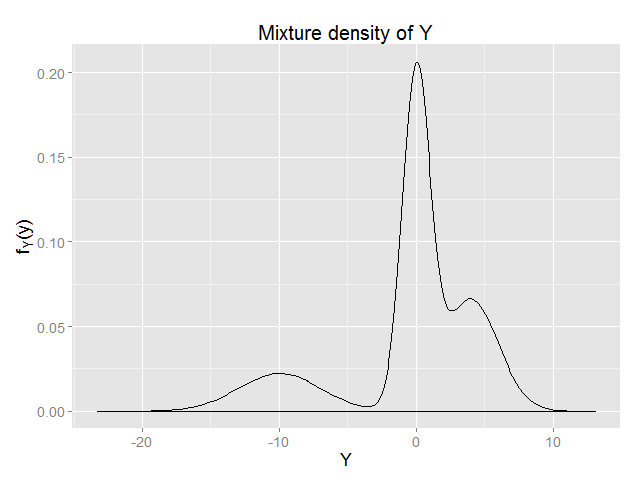
\includegraphics[scale=0.5]{mainmatter/chapter_1_introduction/mixture_density.png}
	\caption{Mixture density of $Y \sim \dfrac{1}{6}N(-10,3) + \dfrac{1}{2}N(0,1) + \dfrac{1}{3}N(4,2)$}
	\label{fig : mixture_density_1}
\end{figure}

Figure \ref{fig : mixture_density_1} shows the density function for $Y$. The density is trimodal with each mode corresponding to one of the components in the mixture. Mixtures like $Y$ which are formed from a finite sum of components are called finite mixtures. The components are also known as mixture components and their densities are called component densities. The constants multiplying their densities are called mixture weights. The mixture weights also represent the probability of selection of each component density. Each mixture weight should be positive and the sum of all mixture weights should be equal to 1. In our example all the  mixture components were having the same parametric family i.e. Normal distribution, but it is also possible to have mixture components from different parametric families (\citealp[pg. 4]{fruhwirth-schnatter_finite_2013}. A mixture model where it is assumed that all data points are generated from a mixture of normally distributed component densities is called Gaussian mixture model (GMM).

\subsection{Formal definition for finite mixture distribution}
\todo[inline]{Mention that we follow notation from \citep{fruhwirth-schnatter_finite_2013} ???}
Given a finite set of probability density functions $p_1(y), p_2(y), \ldots , p_K(y)$ and weights $\eta_1, \eta_2, \ldots , \eta_K$, a random variable $Y$ is said to have a finite mixture distribution if\\
$$p(y) = \sum_{i=1}^{K} \eta_{i} p_{i}(y)$$\\
The vector of the weights $\boldsymbol{\eta} = (\eta_1, \eta_2, \ldots , \eta_K)$ is called the weight distribution. The $k^{th}$ weight $\eta_{k}$ corresponds to selection probability of the $k^{th}$ density while sampling for $Y$. It can only take values from the K dimensional positive real coordinate space ${\mathbb{R}^{+}}^K$ with an additional constraint,\\
$$\sum_{i=1}^{K} \eta_{i} = 1$$\\


\subsection{Issues}
\label{subsec : issues_mixture_density}
One of the biggest challenges while modeling a mixture density for an observed random variable is that the number of mixture components ($K$), weight distribution $\boldsymbol{\eta}$ and the corresponding parameters for component densities might not be known in advance. Another issue is that from a sample of $N$ observations $y_1, y_2, \ldots , y_N$ sampled from the mixture density $p(y)$ one may not know which observation belongs to which component density. Formally, an allocation vector $\boldsymbol{S} = (S_1, S_2,\ldots , S_N)$ represents the allocation of observations to mixture components. i.e. $S_i = k$ represents that $i^{th}$ observation belongs to $k^{th}$ component density. Estimating the allocation vector is in fact solving the clustering problem, albeit using parametric methods in our case. \textcolor{red}{Rephrase the last line}


\subsection{Applications of mixture distribution}
Mixture models have found usage in a variety of domains. Some of the examples are:
\begin{itemize}
\item Spike sorting of neural data: Both GMM and mixture of multivariate t-distributions have been used. \citep{lewicki_bayesian_1994,shoham_robust_2003}.
\item Speaker recognition as well as speech to text conversion algorithms have used mixture models \citep{simancas-acevedo_speaker_2001,xiang_efficient_2003,povey_subspace_2011}.
\item Image processing: GMM have been used to find features in an image like objects, boundaries etc \citep{fu_color_2012}. For e.g. \citet{ming-hsuan_yang_gaussian_1998} have used GMM to model the distribution of skin color pixels. Many authors have also proposed using GMM for face recognition and use it as a biometric identification mechanism.
\item Finance: \citet{brigo_lognormal-mixture_2002} propose to use a lognormal mixture distribution for pricing of financial assets.
\item Biology: Mixture models have found usage in genetics and cell biology.\citep{sim_evaluating_2012,gianola_mixture_2007} 
\end{itemize}

\todo[inline]{I have personally seen NERF researchers using GMM for spike sorting in their lab at IMEC during a visit}

The example applications we cited involved usage of mixture model to adjust for a hidden attribute in the data which could not be collected. However mixtures have also been used as supplementary methodology in various models, a list of which can be found in \citet[pg. 238]{fruhwirth-schnatter_finite_2013}. One such usage in linear mixed models has been proposed by \citet{verbeke_linear_1996} and it also forms the theme of this thesis.

\section{Goal of master thesis}
\label{sec : goal}
\citet*{verbeke_linear_1996} proposed to use a finite mixture distribution of normally distributed components for the prior distribution of random effects in a linear mixed effects model(LMM). \textcolor{red}{Refer to a section}. This linear mixed effects model is also known as Heterogeneity model. For the scope of this thesis our focus will be on the bayesian version of the linear mixed effects model(BLMM), where all parameters involved are assigned a probability distribution. However in both types of models one has to tackle the issues described in section \ref{subsec : issues_mixture_density}. The aim of this master thesis is to evaluate existing approaches \textcolor{red}{name some approaches like marginal likelihood etc.} for solving these issues. Since we will be following the bayesian paradigm, we will use MCMC methods instead of the frequentist point estimation methods. While we will use the longitudinal data set \textcolor{red}{[name of the data set here]} to fit bayesian linear mixed effect model, we will also simulate data sets to compare various approaches for choosing the number of components.